\section{Resumen}
La base de conocimiento colaborativo Wikidata \cite {vrandevcic2014wikidata} es el almacenamiento central de los datos estructurados asociados con los  proyectos de Wikimedia. Wikidata es una base de datos no relacional, donde se representa la información en forma de grafo dirigido; donde los nodos son entidades y las aristas son relaciones. En este documento se intenta estudiar si basado en ese grafo se puede medir la similitud de dos entidades. Las preguntas principales que se intentan responder en este trabajo son: ¿Se puede aplicar métricas de similitud aplicadas en otros grafos?, ¿Qué deben de tomar en consideración estas métricas para realizar una buena medición de la similitud?.

Al finalizar esta investigación se pretende responder las preguntas anteriores revisando bibliografía relacionada, donde se espera encontrar y clasificar distintas métricas, y compara sus resultados con una escala base de similitud, para determinar cuál es la mejor forma de medir la similitud tomando como casos las métricas anteriormente clasificadas.  
\section{Introducción}
Wikidata contiene más de 45 millones de elementos de datos \cite{balaraman2018recoin}. Actúa como el centro de interconexión de las páginas de Wikipedia sobre un elemento específico en diferentes idiomas. Automatiza funciones como las infoboxes en Wikipedia y se utiliza cada vez más para otras aplicaciones, como el enriquecimiento de datos y la respuesta a preguntas.

Wikidata es una base de datos no relacional, la cual está formada por entidades (nodos) y relaciones
(aristas) que unen las entidades  \cite{vrandevcic2014wikidata}. Al buscar en Wikidata nos encontramos con entidades que al  parecer son similares, ¿Pero son similares? O ¿Soló es mi percepción de las entidades?, es aquí donde nos surge la necesidad de una escala uniforme para medir la similitud  de dos entidades, y de esta
manera poder decir “Con base en la escala \textit{x} estas dos entidades son muy similares”. Al medir la similitud entre entidades, se puede utilizar este dato para encontrar entidades duplicadas, además  se puede utilizar para apoyar algoritmos recomendadores  y clustering.

Ahora por la naturaleza de Wikidata, esto se podría hacer de diferentes maneras. En las siguientes  imágenes  se muestra parte de la información sobre los poetas Pablo Neruda (PN), Gabriela Mistral (GM) y Gabriel García Márquez (GGM).

\begin{figure}[ht]
\centering
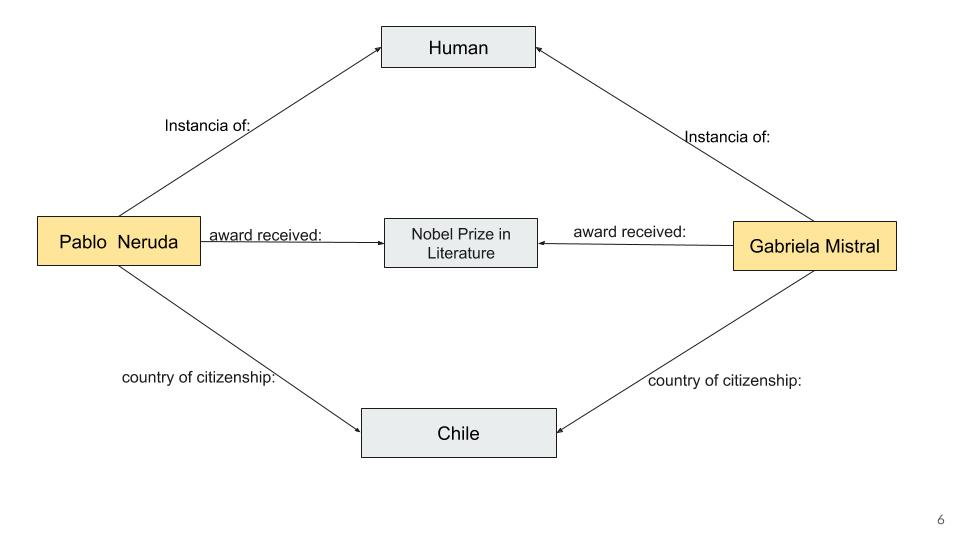
\includegraphics[scale=0.3]{Imagen1.jpg}
\label{fig:Imagen1 }
\caption{Información de Pablo Neruda y Gabriela Mistral}
\end{figure}


\newpage

Considerando solo esta información, ¿Cómo podemos determinar quien es más similar a Pablo Neruda? ¿Gabriela Mistral ó Gabriel García Márquez? ¿Qué significa la noción de similitud aquí? ¿Se puede crear un método automatizado que puede capturar esta noción?   Para responder estas preguntas, una noción simple de analizar es ver a que distancia se encuentran los autores; sin embargo si nos centramos en la Figura 1 y tomamos las aristas como no dirigidas, vemos que  entre Pablo Neruda y Gabriela Mistral existen 3 caminos distintos de tamaño 1 (número de nodos), por lo que tomar esta métrica no es buena idea, ya que todos los humanos tendrán una similitud igual a 1.


Otra métrica que se puede utilizar, es  contar los vecinos comunes entre las entidades, por lo que la  similitud(PN,GM)= 3 y similitud(PN,GGM)=2; pero  ¿Cómo se modifica estos valores si agregamos más información, por ejemplo el sexo de las personas?

\begin{figure}[ht]
\centering
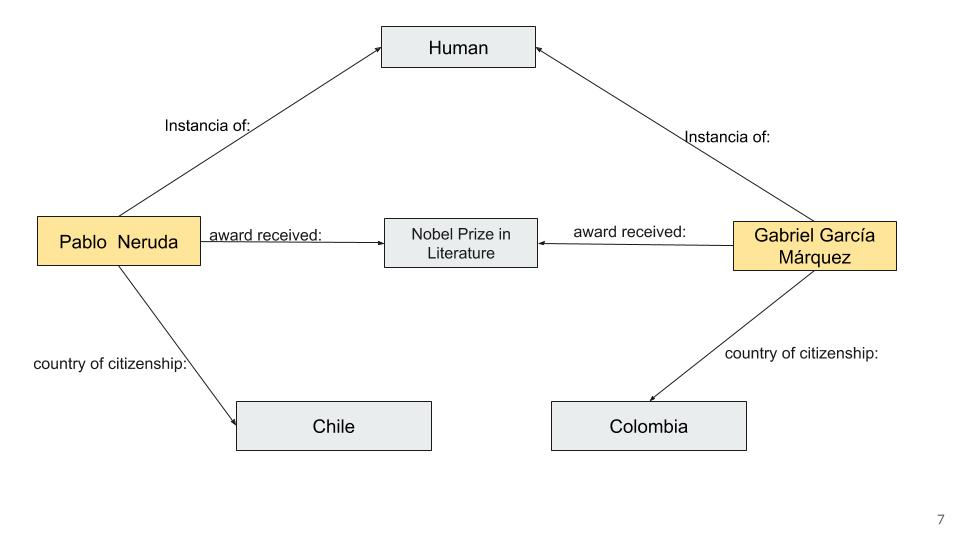
\includegraphics[scale=0.3]{Imagen2.jpg}
\label{fig:Imagen2 }
\caption{Información de Pablo Neruda y Gabriel García Márquez}
\end{figure}

\newpage
\subsection{Método Vecinos Comunes}
Este método fue utilizado  \cite{newman2001clustering}  en el estudio de redes de colaboración, mostrando una correlación positiva entre el número de vecinos comunes y la probabilidad de que dos científicos colaboren en el futuro; concluyendo que la probabilidad de colaboración entre científicos  en función de su número de conocidos mutuos en la red está fuertemente correlacionada positivamente.




El método de calcular los vecinos comunes podría servir para calcular la similitud, pero  ¿Qué pasará si en vez de tomar los nodos, nos centramos en las aristas? Para hacer esto se puede partir del hecho de que las instancias de humanos son muchas más que las personas con nacionalidad chilena, y el grupo de personas que han ganado el premio nobel de literatura es el grupo  menos numeroso; y basándonos en esto se le asigna pesos como los de la Figura 3. 


Notando que la arista que va desde cada poeta a Humano tiene un valor menor que la arista que va de  un poeta a Chile; esto se puede interpretar como que  dos entidades que son de la clase Humano tienen una similitud = 0.2 (por ejemplo), solo por el hecho de ser de la misma clase, y dos humanos que tienen nacionalidad Chilena tiene más similitud = 0.5 por pertenecer a un mismo país, pero dos poetas que han ganado el premio nobel de literatura serán mucho más similares, ya que es un grupo más reducido. 

Si tomamos estos dos últimos métodos (vecinos comunes, pesos a las aristas) surgen las siguientes incógnitas ¿Qué método es mejor? ¿Es mejor el método que se basa en los nodos, que el que toma las aristas como referencia? ¿Cómo se pueden comparar los resultados de varios métodos?  

Si bien la noción de similitud es bastante subjetiva, este estudio se basa en la información presente en Wikidata, tomando el hecho de que está información está representada en forma de grafo, donde se puede aplicar algoritmos que intenta aproximarse a esta noción. 
 
\begin{figure}[h]
\centering
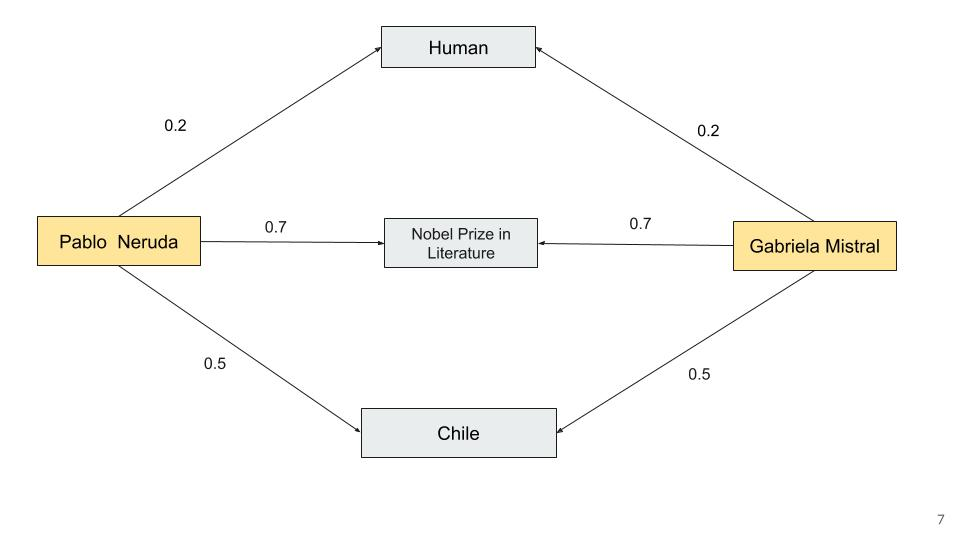
\includegraphics[scale=0.3]{Imagen3_1.jpg}
\label{fig:Imagen3 }
\caption{Ejemplo de asignación de pesos}
\end{figure}
 
\newpage
\section{Trabajos Relacionados}
Existe un  estudio comparativo \cite{lu2011link} donde se encuentran diferentes algoritmos de similitud aplicados en grafos; cabe recalcar que estos  algoritmos son aplicados a grafos no dirigidos, sin embargo es un buen punto de partida para comenzar nuestra investigación, ya que en el se encuentra un buen banco de algoritmos de similitud  y algunas aplicaciones de estos.    

Un método  interesante a analizar es el  método Vertex \cite{leicht2006vertex} el cual propone  una medida de similitud basada en el concepto de que dos vértices son similares si sus vecinos inmediatos en la red son similares; además se nos muestra la aplicación de este método a ciertos problemas, como por ejemplo  encontrar sinónimos en un diccionario basándose en su definición; concluyendo que los  resultados parecen indicar que la medida es capaz de extraer información útil sobre la similitud de los vértices en función de la topología de la red.

Relacionado a la anterior, en  \cite{sinha2007unsupervised} se presentan evaluaciones comparativas usando varias medidas de la similitud semántica de las palabras y varios algoritmos para la centralidad de los grafos. Los  resultados indican que la combinación correcta de métricas de similitud y algoritmos de centralidad de grafos puede, conducir a un rendimiento que compita con el estado del arte en la desambiguación del sentido de la palabra no supervisada, medida en conjuntos de datos estándar.

Otro algoritmo importante de recalcar es SimRank \cite{jeh2002simrank}  el cual propone un enfoque complementario, aplicable en cualquier dominio con relaciones de objeto a objeto, que mide la similitud del contexto estructural en el que se producen los objetos, en función de sus relaciones con otros objetos; es decir, es  una medida que dice: dos objetos son similares si están relacionados con objetos similares.

SimRank fue utilizado en \cite{fogaras2005scaling} para explotar la información de similitud oculta en la estructura de enlaces de la web; este documento presenta algoritmos escalables a grafos con miles de millones de vértices en una arquitectura distribuida. La similitud de los barrios de vértices de varios pasos se evalúa numéricamente mediante funciones de similitud que incluyen SimRank , un refinamiento recursivo de la cocitación; PSimRank, una nueva variante con mejores características teóricas; y el coeficiente de Jaccard, extendido a barrios de pasos múltiples. Los resultados experimentales sugieren que la estructura de hipervínculo de los vértices dentro de cuatro a cinco pasos proporciona información más adecuada para la búsqueda de similitud que los vecindarios de un solo paso.

En cuanto a la relación semántica y la desambiguación \cite{hulpucs2015path}, se ha abordado  dos problemas fuertemente interdependientes: la relación semántica y la desambiguación. El objetivo de la relación semántica es ponderar las asociaciones semánticas entre pares de conceptos. El objetivo de la desambiguación de entidad y palabras clave es vincular cadenas en el texto con los conceptos correspondientes, donde para hacer esto se utilizaron varios algoritmos de similitud. 

Otra aplicación de la similitud la encontramos en \cite{calado2006link}, donde los autores evalúan cómo se puede usar la estructura de enlace de la web para determinar una medida de similitud apropiada para la clasificación de documentos. Experimentan con cinco medidas de similitud diferentes y determinan su adecuación para predecir el tema de una página web. Las pruebas realizadas en un directorio web muestran que la información del enlace por sí sola permite clasificar los documentos con una precisión promedio del $86 \% $. Además, cuando se combina con un clasificador tradicional basado en texto, la precisión aumenta a valores de hasta $90 \%$. Debido a que las medidas propuestas en este artículo son sencillas de calcular, proporcionan una solución práctica y efectiva para la clasificación de documentos de la Web y las tareas de recuperación de información relacionadas. 

Un estudio cercano al nuestro es el medir la completitud de la información en Wikidata \cite{balaraman2018recoin}, donde se intenta medir que tan completa es la información en esta base de datos; para esto se mide la cantidad de información que hay para cada entidad respecto a entidades similares, es decir que tanta información hay de Alexis Sanchez (Futbolista Chileno) respecto a los datos de los otros jugadores en Wikidata; si bien en este trabajo se utiliza el concepto de entidades similares, lo hace de una manera básica; se basa solamente en que dos entidades son similares si son del mismo tipo (Países con Países, Cuidades con Cuidades), y  si son de tipo Humano dos entidades son similares si son de la misma profesión (petas con poetas, futbolistas con futbolista).

\section{Objetivos e Hipótesis}
Los índices de similitud en bases de datos de grafos se pueden clasificar de diferentes maneras \cite{lu2011link}, sin embargo podemos diferenciar dos grupos, primero están los algoritmos que se basan en los nodos vecinos, es decir son algoritmos que se mueven a través del grafo utilizando las aristas, pero ignoran que representa está arista. Segundo  son algoritmos que  utilizan la información de la arista, no solo se mueven a través de ella como un simple camino, sino que usan la información que la arista provee.
 
Ejemplificando lo anterior podemos ver en la Figura 1  que el método de vecinos comunes encontrará que la entidad de \textbf{Nobel Prize in Literature} es común entre Pablo Neruda y Gabriela Mistral, pero esté ignoro que la arista representa la relación \textbf{award received}  y que está podría sumar más a la similitud de las dos entidades, sin embargo se cuenta igual que la relación \textbf{instance of} ya que \textbf{Human} también  es vecino común.

Ahora por la naturaleza de Wikidata las relaciones representan información importante a considerar, por lo que  las siguientes preguntas son importante  ¿Son mejores los algoritmos de similitud que utilizan la información de las aristas? ¿Se puede aplicar o adaptar los algoritmos utilizados en grafos simples (no dirigidos y sin información en la arista) a Wikidata?

Algo importante a considerar al manejar un algoritmo es su escalabilidad, más aún trabajando en una  base de datos tan grande como Wikidata, por lo que también en este estudio se pretende hacer énfasis en este aspecto, si existen algoritmos que proveen una buena medición de la similitud pero no son escalables.   

  
\subsection{Objetivo General}
\begin{itemize}
\item Adaptar, aplicar y comparar algoritmos  de similitud de entidades en Wikidata.   
\end{itemize}  

\subsection{Objetivos Específicos}
\begin{itemize}
\item Adaptar algoritmos de similitud aplicados en otros grafos  a  Wikidata.
\item Aplicar algoritmos que ignoren la información de las aristas en Wikidata. 
\item Aplicar algoritmos que si utilicen la información de las aristas. 
\item Compara los resultados de los algoritmos respecto a su escalabilidad. 
\item Compara los resultados de los algoritmos respecto a las similitudes que encuentran.
\end{itemize}
\subsection{Hipótesis}
\begin{itemize}
\item Es posible adaptar algoritmos utilizados en otro tipo de grafos a Wikidata. 
\item  Los métodos que  utilizan la información de las aristas medirán mejor\footnote{ver definición de mejor en el sección de metodología; página 9} la similitud que los métodos que solo se basan en la información de los nodos. 
\end{itemize}
\subsection{Preguntas de Investigación}
\begin{itemize}
\item ¿Es posible adaptar algoritmos utilizados en otro tipo de grafos a Wikidata?
\item ¿Son los métodos que  utilizan la información de las aristas mejores que los métodos que solo se basan en la información de los nodos para medir la similitud en Wikidata?
\end{itemize}

\section{Metodología}
Las actividades a realizar aparecen en la figura 4. 
 \begin{figure}[h]
 \centering 
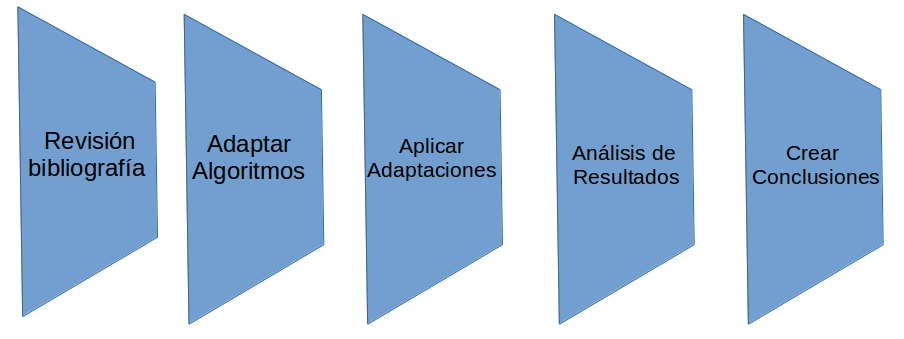
\includegraphics[scale=0.3]{esquema2.jpg}
\label{fig:Imagen4 }
\caption{Pasos a seguir}
\end{figure}


\begin{enumerate}
\item \textbf{Revisión bibliografía}: Se comenzará buscando métricas de similitud aplicados en otros grafos, considerando su escalabilidad y su posible aplicación a Wikidata. 

\item \textbf{Adaptar Algoritmos}:  En este punto se trabajara con datos de Wikidata, pero en un dominio especifico, para así poder realizar las adaptaciones de los algoritmos de forma más fácil y rápida; y de esta manera asegurarse que los algoritmos funcionen correctamente.
 

\item  \textbf{Aplicación de Adaptaciones}:  Aquí se realizarán mediciones de similitud de entidades con una cantidad de datos mayor, no se puede asegurar que con la totalidad de los datos, ya que se puede encontrar con algoritmos que su costo es alto, pero la métrica tiene un importante aporte a nuestro estudio.

\item \textbf{Análisis de Resultados}: Se procederá a compara los resultados de la etapa anterior con respecto al rendimiento y similitud que encuentran los algoritmos. 

\item \textbf{Crear Conclusiones}: Se crearán conclusiones que intenten responder a las preguntas de investigación. 
\end{enumerate}
\newpage
Al intentar determinar  cuál es el mejor algoritmo midiendo la similitud, surge el problema de  no tener una escala base para comparar los resultados \cite{leicht2006vertex}, por lo que se propone las siguientes alternativas para tener una base de comparación.

\begin{itemize}
\item \textbf{Consulta a Usuarios:} En un inicio elegir un dominio (películas, libros,etc) y luego crear una encuesta para consultar a usuarios ¿Qué elementos les parecen similares?; esta opción tiene un inconveniente, ya  que la creación del instrumento de consulta puede ser complejo y ocupe demasiado tiempo, lo que nos limita en la prueba de las métricas que es nuestro objetivo principal.  
\item \textbf{Utilizar data-set de recomendares}: De igual manera utilizaremos un dominio especifico, y se buscará un data-set para entrenar un recomendador. Un ejemplo de estos puede ser el data-set “More Ninja” que presenta https://movielens.org/, el cual es el resultado de un algoritmos de recomendación, basado en similitud de películas tomando como parámetros menos violentas, más realistas, entre otros.
Si bien esta opción se basa en gusto de los usuarios, y aún así se mantiene cierta
subjetividad, esta opción nos da un plus a nuestra investigación, ya que contrastaríamos una sistema recomendador, con un algoritmos de similitud aplicado a un grafo; dicho de otra manera, veremos si podemos llegar al mismo resultado de similitud sin considerar la información de los usuarios, solo basado en el grafo mismo.
\item \textbf{Diccionario de Sinónimos:} Se tomará conceptos parecidos como ser los pares (car,automobile) o (music, melody)  basado en un diccionario de sinónimos; esto de igual manera nos podría sumar, ya que estaríamos haciendo un estudio semántico de sinónimos; con la información en Wikidata usando técnicas de similitud.
\end{itemize}